\chapter{Introduction}

\section{Sequencing Technologies in Cancer Research}

% Las secuencias genómicas ejercen elevada influencia sobre la biología de los 
% organismos y permiten inferir su historia evolutiva. 


% SECUENCIAS GENOMICAS Y MEDICINA DE PRECISIÓN

Genomic sequences significantly influence organismal biology and provide 
insights into evolutionary history. The application of this genomic knowledge 
to human health has given rise to precision medicine, a discipline that 
leverages genetic and molecular markers to personalize medical treatments 
according to individual patient characteristics \cite{collins_new_2015}. 
Advances in sequencing platforms and bioinformatics tools have enabled the 
identification of genetic variations that predispose individuals to specific 
diseases, facilitating the design of targeted therapies that enhance efficacy 
while reducing side effects \cite{carrasco-ramiro_human_2017}.

In oncology, genomic analyses have revolutionized our understanding and 
therapeutic approach to cancer \cite{johannessen_progress_2017}. According to 
the National Cancer Institute (NCI), cancer encompasses more than 100 distinct 
types, arising when normal cells undergo genetic and/or epigenetic alterations 
leading to uncontrolled proliferation and compromised organismal homeostasis
\cite{nci_what_2007}. Cancer development represents a complex process resulting 
from interactions between individual genotype and various environmental 
factors, driving clonal evolution where distinct malignant cell subpopulations 
compete for resources and space \cite{turajlic_resolving_2019}. Tumor DNA 
sequencing enables identification of patient-specific driver mutations, 
facilitating more effective targeted therapy selection and implementation 
\cite{sicklick_molecular_2019}.

% Las secuencias genómicas ejercen una elevada influencia sobre la biología de los 
% organismos y permiten inferir su historia evolutiva. La aplicación de esta 
% información en el ámbito de la salud humana ha dado lugar a lo que se conoce 
% como medicina de precisión. Esta disciplina, mediante el uso de marcadores 
% genéticos y moleculares, permite personalizar los tratamientos médicos, 
% adaptándolos a las características individuales de cada paciente. Gracias a los 
% avances en las plataformas de secuenciación y de herramientas bioinformáticas,
% es posible identificar variaciones genéticas que predisponen a ciertas 
% enfermedades y diseñar terapias específicas que mejoran la eficacia y reducen 
% los efectos secundarios.

% En el contexto del cáncer, los análisis genómicos han revolucionado nuestra 
% comprensión y abordaje terapéutico de la enfermedad. El cáncer, que engloba 
% más de 100 tipos diferentes según el Instituto Nacional del Cáncer (NCI), surge 
% cuando las células normales experimentan alteraciones genéticas y/o epigenéticas 
% que las llevan a proliferar de forma descontrolada, comprometiendo la 
% homeostasis del organismo. Su desarrollo es un proceso complejo que resulta de 
% la interacción entre el genotipo del individuo y diversos factores ambientales, 
% dando lugar a una evolución clonal donde distintas subpoblaciones de células 
% malignas compiten por recursos y espacio. La secuenciación del ADN tumoral 
% permite identificar las mutaciones específicas que impulsan el crecimiento 
% canceroso en cada paciente, facilitando la selección de terapias dirigidas más 
% efectivas.

DNA sequencing methods have evolved significantly over the years, with current 
technologies falling into three main categories:

\begin{itemize}[label=\tiny\raise.5ex\hbox{•}, leftmargin=\parindent]
    
    \item \textbf{Chain-termination method}: Also known as Sanger sequencing 
    after its primary developer, this technique relies on controlled DNA synthesis 
    termination, generating fragments of varying lengths that reveal the original 
    sequence when size-separated. While largely superseded for genomic projects 
    due to its low throughput, it remains valuable in research for verifying 
    short reads such as PCR products from individual genes 
    \cite{moorcraft_understanding_2015}.

    \item \textbf{Short-read sequencing}: Technologies that perform massive 
    parallel sequencing of clonally amplified DNA fragments (250-600 bp), 
    delivering high sequencing depths with $>$99.9\% accuracy
    \cite{logsdon_long-read_2020}. Illumina dominates this category globally, 
    though recent years have seen competition from MGI Tech, which promises 
    faster, more cost-effective high-quality sequencing
    \cite{jeon_comparison_2021}.

    \item \textbf{Long-read sequencing}: This approach also employs parallel 
    sequencing strategies but generates individual reads spanning tens to 
    thousands of kilobases. Currently, two main methods dominate this field: 
    Single Molecule Real-Time (SMRT) sequencing, commercialized by PacBio, and 
    nanopore sequencing, pioneered by Oxford Nanopore Technologies (ONT) 
    \cite{logsdon_long-read_2020} with the recent appearence of MGI Tech as
    possible alternative \cite{zhang_single-molecule_2024}.

\end{itemize}

\subsection{Limitations of Short-read Genome Assembly}

Cancer is largely driven by somatic changes in the genome, which can range from 
small nucleotide substitutions to chromosome-scale rearrangements. In this context, 
sequencing technologies play a crucial role, with predominant short-read sequencing 
having revolutionized our understanding of point mutations. However, this 
approach proves insufficient for resolving most large genomic alterations and 
generating gap-free assemblies. This limitation stems from the inherent 
inability of short reads (typically 150-300 base pairs) to span complex genomic 
regions, particularly those containing repetitive elements or large structural 
variations \cite{ho_structural_2020}. Furthermore, the fragmented nature of short 
reads complicates the accurate reconstruction of complex genomic architectures, 
often leading to ambiguous or incomplete assemblies 
(\textbf{Figure~\ref{fig:assembly_gaps}}).

\begin{figure}[H]
    \centering
    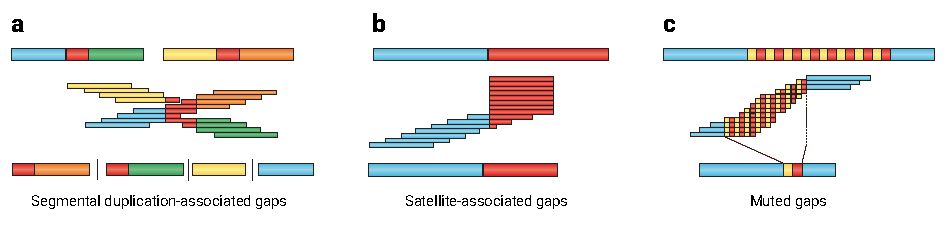
\includegraphics[width=\textwidth]{img/assembly_gaps.pdf}
    \caption[Limitations of short-read genome assembly]{Limitations of short-read 
    genome assembly. The upper bar of each figure shows regions to be resolved, 
    with repetitive sequences highlighted in red. The middle displays 
    short-read alignments, while the bottom bar shows the inferred sequence. 
    (\textbf{a}) Large segmental duplications of high sequence identity (orange 
    and green) create ambiguous read overlaps, resulting in multiple gaps flanking 
    segmental duplications. (\textbf{b}) Satellite-associated gaps represent 
    a special case causing read 'pileups' due to higher-order tandem arrays of 
    repetitive sequences, primarily occurring in centromeric, acrocentric, and 
    telomeric genomic regions. (\textbf{c}) Muted gaps occur when the assembled 
    sequence appears shorter than the actual genome, typically in repetitive 
    regions that are difficult to amplify or are toxic to bacterial cloning, 
    such as simple tandem repeats. Adapted from \cite{chaisson_genetic_2015}.}
    % \caption[Algunas limitaciones en ensamblajes genómicos con lecturas cortas]{
    % Algunas limitaciones en ensamblajes genómicos con lecturas cortas. Encima De
    % cada figura están representadas las regiones a ser resueltas y las zonas
    % coloreadas de rojo son secuencias repetitivas. En medio de cada figura se 
    % muestran los alineamientos de lecturas cortas, y abajo del todo se encuentra
    % la secuencia que se ha sido inferida. (a) Large segmental duplications of 
    % high sequence identity, in orange and green, make read overlaps ambiguous, leading
    % to multiple gaps flanking segmental duplications. The effect becomes exacerbated 
    % if the duplications are structurally polymorphic in a diploid genome. (b)
    % Satellite-associated gaps are a special case leading to read ‘pileups’ due 
    % to higher-order tandem arrays of repetitive sequence, These occur primarily in centromeric,
    % acrocentric and telomeric areas of genomes. (c) Muted gaps arise when the 
    % assembly is contracted relative to the true genome when overlaps are consistent 
    % with a smaller representation of the genome. These are often associated with
    % repetitive sequences that cannot be easily amplified and/or are incompatible 
    % with cloning and propagation (that is, when they are toxic to Escherichia coli), 
    % such as simple tandem repeats.}
    \label{fig:assembly_gaps}
\end{figure}

\subsection{Long-read Contributions to Genome Assembly}

Long-read sequencing technologies emerged a decade ago, marking a turning point 
in sequence assembly by addressing short-read limitations. Initially, these 
technologies had much higher error rates (~10\%) compared to short reads ($<$ 1\%)
\cite{espinosa_advancements_2024}. While this enabled routine bacterial genome 
assembly, it limited their application in human genomics, particularly for point 
mutation detection \cite{loman_complete_2015}. However, continuous improvements 
in long-read sequencing platforms have progressively reduced these error rates, 
ultimately enabling the generation of the first gap-free human reference genome, 
known as telomere-to-telomere (T2T) assembly \cite{nurk_complete_2022}. 
This achievement resolved previously inaccessible genomic regions that remained 
incomplete in the Genome Reference Consortium's human reference version 38 
(GRCh38), highlighted in red in \textbf{Figure~\ref{fig:T2T_ref}}.

% The advent of Las tecnologías de secuenciación de lecturas largas hace una
% década con el potencial de superar las limitaciones de las lecturas cortas,
% and marked a turning point in sequence assembly. Sin embargo, esas long reads 
% tenían higher error rate (~10\%) than short reads ($<$ 1\%), it was practical to 
% routinely assemble complete bacterial genome, pero desincentivaba su uso
% en genómica humana debido a no ser útiles en el análisis de mutaciones puntuales.
% No obstante, las continuas mejoras de las plataformas de secuenciación basadas
% en long-reads han ido reduciendo estos error rates, hasta el punto de permitir 
% generar el primer genoma humano de referencia sin gaps, también denominado 
% telómero a telómero (T2T), adressing genomic regions remained unresolved in the
% la versión 38 de la referencia humana lanzada por el Genome Reference Consortium
% (GRCh38).

\begin{figure}[H]
    \centering
    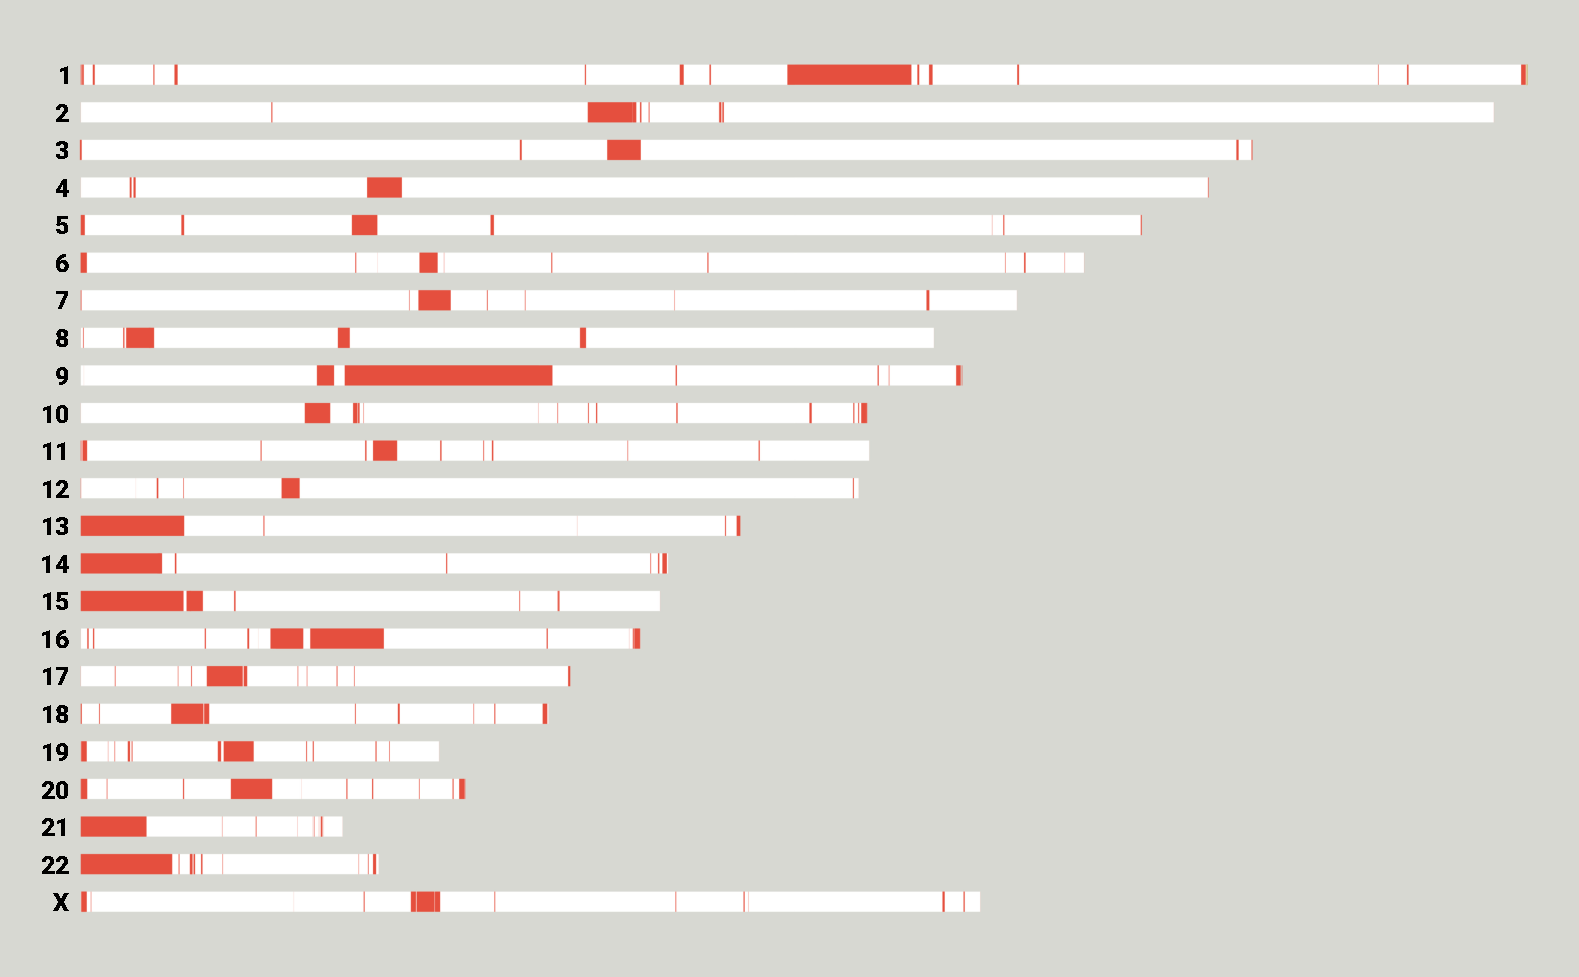
\includegraphics[width=\textwidth]{img/T2T_ref.pdf}
    \caption[Gaps resolved by T2T assembly]{Gaps resolved by T2T assembly. Each 
    bar represents a linear visualization of a chromosome, with chromosome 
    numbers indicated on the left. Red segments denote previously missing 
    sequences resolved by the T2T Consortium in 2022. The Y chromosome is not 
    included, as its complex architecture, particularly its large, tandemly 
    arrayed and inverted repeats (IRs), required additional analysis and was 
    published separately in 2023 \cite{rhie_complete_2023}. Adapted from 
    \cite{zahn_filling_2022}.}
    % \caption[Gaps resolved by T2T assembly]{Gaps resolved by T2T assembly. 
    % Each bar is a linear visualization of a chromosome, with the chromosome 
    % number shown at left. Red segments denote previously missing sequences that 
    % the T2T Consortium resolved in 2022. No se incluye el cromosoma Y, debido
    % a que fue publicado posteriormente en 2023 debido a su compleja arquitectura,
    % specifically the presence of large, tandemly arrayed and inverted repeats (IRs).}
    \label{fig:T2T_ref}
\end{figure}

Beyond sequencing methodology, significant differences exist between long-read 
platforms. Although PacBio pioneered the field in 2011 with high-throughput 
sequencing systems, their platforms have consistently required investments in 
the hundreds of thousands of dollars. In contrast, ONT's 2014 launch of MinION 
introduced a low-throughput but highly portable device requiring only a few 
thousand dollars investment. Subsequently, ONT expanded into high-throughput 
PromethION devices, notably the ``P2 solo'' model, which enables Whole Genome 
Sequencing (WGS) with a computer connection at under \$20,000. This 
cost-effective solution makes long-read sequencing accessible to virtually any 
molecular biology laboratory \cite{espinosa_advancements_2024,noauthor_vega_nodate,oxford_nanopore_technologies_nanopore_nodate}.

ONT sequencing technology operates by measuring ionic current changes as 
single-stranded DNA molecules thread through nanoscale pores embedded in a 
membrane. Each nucleotide's unique shape creates distinctive current 
perturbations as it passes through the pore, enabling sequence determination 
and even modified bases detection. These nanopores are arranged in arrays across 
a flow cell, ONT's core consumable component, which contains thousands of 
individual sensing channels. Each flow cell integrates microfluidics for sample 
delivery, electronics for current measurement, and an application-specific 
integrated circuit (ASCI) that enables real-time data collection from multiple 
nanopores simultaneously (\textbf{Figure~\ref{fig:ont_seq}}). 

\begin{figure}[H]
    \centering
    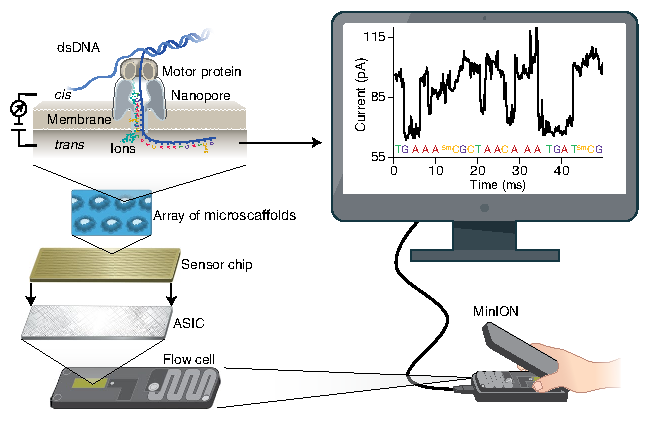
\includegraphics[width=0.8\textwidth]{img/ont_seq.pdf}
    \caption[Principle of nanopore sequencing]{Schematic representation of 
    nanopore sequencing using MinION technology. The diagram shows the key 
    components: nanopore embedded in a membrane, array of microscaffolds, 
    sensor chip, ASIC, and flow cell. The ionic current measurement graph 
    displays the characteristic signal patterns produced as DNA strands pass 
    through the nanopore. Adapted from \cite{wang_nanopore_2021}.}
    \label{fig:ont_seq}
\end{figure}

Recent improvements in both the nanopore architecture of flow cells 
(transitioning from the R9 pore protein, with a 9 Å constriction, to the R10 
variant featuring a longer barrel and 10 Å constriction) and basecalling 
algorithms have significantly enhanced sequence accuracy 
(\textbf{Figure~\ref{fig:ONT_updates}}), making long-read sequencing a viable 
approach for the systematic analysis of cancer-associated variation
\cite{kolmogorov_scalable_2023,sakamoto_phasing_2022,schaal_migrating_2022}.

\begin{figure}[H]
    \centering
    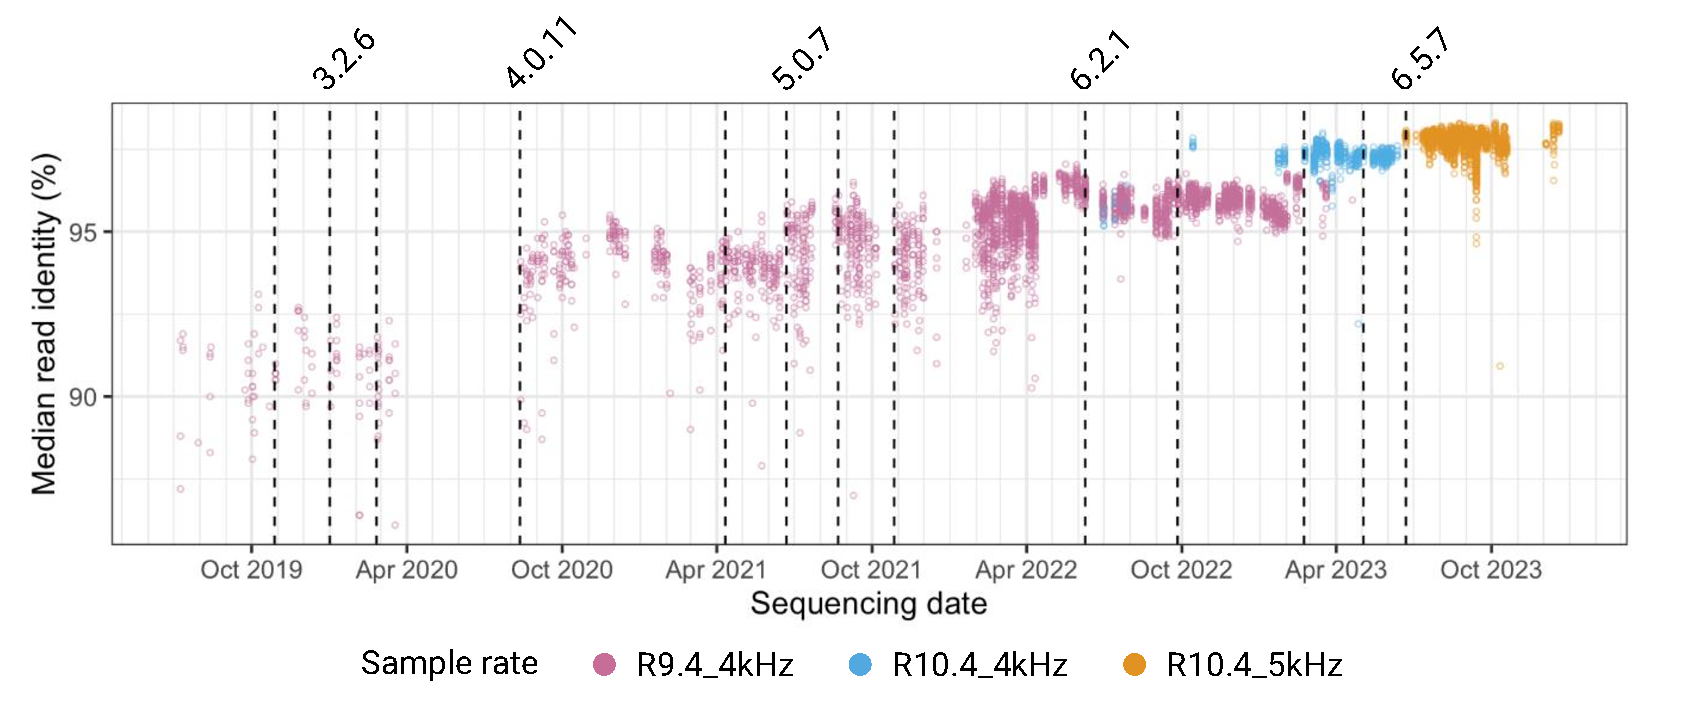
\includegraphics[width=\textwidth]{img/ONT_updates.pdf}
    \caption[Evolution of ONT basecalling accuracy]{Temporal evolution of median 
    read accuracy using Oxford Nanopore's Guppy basecaller versions shown 
    above. Each data point represents a human WGS experiment at 20-30x coverage 
    depth. Colors indicate the flowcell version and sampling rate: R9.4\_4kHz 
    (pink), R10.4\_4kHz (blue), and R10.4\_5kHz (orange), where sampling rate 
    (kHz) represents the number of electrical measurements per second during 
    sequencing (1 kHz = 1,000 measurements per second). Data from Genomics 
    England's R\&D Department, presented in ONT's Webinar ``Unlocking 
    comprehensive genome for large-scale projects'', courtesy of Adam Giess and 
    Melanie Tanguy \cite{oxford_nanopore_technologies_unlocking_2024}.}
    \label{fig:ONT_updates}
\end{figure}

The assembly of the first T2T genome required inputs from multiple platforms: 
PacBio for long and accurate HiFi data (15--25 kb at 99.5\% accuracy), 
ONT for ultra-long (UL) data ($>$100 kb at 95\% accuracy), and Illumina' 
short-reads (0.15 kb at 99.99\% accuracy) \cite{li_genome_2024}. While this 
combination of data types proved effective, it complicated data generation and 
limited accessibility. Currently, ONT provides all three sequencing modes on a 
single instrument using R10.4 PromethION flow cells, specific assembly chemistry 
kits, and associated bioinformatic workflows, resulting in automated assemblies 
with base accuracy exceeding 99.999\% and near-perfect continuity
\cite{koren_gapless_2024}. This is particularly promising as it opens up the 
possibility of generating personalized human genomes using PromethION sequencers 
for precision medicine research purposes.

\subsection{Structural Variation in Cancer}

Structural variants (SVs) are genomic alterations ranging from 50 pb to 
whole-chromosome events, including deletions, insertions, and segment 
rearrangements. The significance of SVs as a hallmark of cancer is becoming 
increasingly evident. A recent analysis of 2,658 tumor genomes revealed that 
approximately 50\% of driver mutations overlap with SVs, highlighting their 
crucial role in cancer development \cite{li_patterns_2020,menghi_tandem_2018}. 
Despite their importance as biomarkers in oncological diseases, our 
understanding of SVs remains limited compared to single nucleotide variants 
(SNVs). This knowledge gap stems primarily from the technical limitations of 
short-read sequencing, which has dominated large-scale genome sequencing 
projects. Using short reads, SV detection mainly relies on copy number variation 
(CNV) estimates, an indirect measure that fails to capture copy-number neutral 
events, inversions, and balanced translocations. Consequently, many 
cancer-driving SVs escape discovery using traditional short-read sequencing 
\cite{cameron_comprehensive_2019,abel_mapping_2020}.

The emergence of long-read sequencing technologies has marked a turning point in 
SV analysis, enabling improved variation detection in cancer genomes. A pioneering 
study using medulloblastoma cells, a primary childhood brain tumor, analyzed samples 
at diagnosis and post-treatment using long-read sequencing. This approach led to 
the identification of a novel mutational pattern called templated insertion (TI) 
thread, characterized by short ($<$1 kb) insertions that self-concatenate into highly 
amplified structures up to 50 kbp in size. This pattern was subsequently confirmed 
in other cancer types, showing particular prevalence in liposarcomas and frequent 
co-occurrence with chromothripsis, a catastropic mutational event where 
chromosomes shatter and reassemble chaotically \cite{rausch_long-read_2023}.

Long-read sequencing has also enabled the characterization of novel mutation 
mechanisms driving genomic rearrangements in cancer. A notable example is the 
discovery of loss-translocation-amplification (LTA) chromothripsis in osteosarcoma. 
This mechanism, initiated by a single double-strand break, triggers simultaneous 
TP53 inactivation and oncogene amplification through breakage-fusion-bridge cycles. 
LTA chromothripsis appears to be uniquely prevalent in osteosarcoma, distinguishing 
it from other TP53-driven cancers \cite{valle-inclan_ongoing_2025}.

\subsubsection{Multiple Myeloma as a Model for SVs Detection}

Multiple myeloma (MM) is a neoplasm of terminally differentiated B cells (plasma 
cells) characterized by frequent chromosomal translocations that place oncogenes 
under the control of immunoglobulin enhancers. Unlike most hematopoietic cancers, 
MM exhibits complex chromosomal abnormalities. Some of these SVs, first detected 
more than two decades ago, remain major prognostic factors 
and are currently used for risk stratification in MM patients, primarily through 
Fluorescence in situ hybridization (FISH) detection \cite{kuehl_multiple_2002}.

MM follows a characteristic remission/relapse cycle where cancer cells progressively 
acquire resistance to different lines of treatment (\textbf{Figure~\ref{fig:evo_MM}})
\cite{kurtin_relapsed_2013}. In this context, ONT nanopore sequencing combined 
with automated SV calling methods could enhance our understanding of disease 
mechanisms and potentially identify new prognostic markers and treatment 
targets, ultimately contributing to improved patient care and survival outcomes. 
However, evaluating these strategies remains challenging due to two limitations: 
the lack of a golden standard for SV calling and the absence of curated, open 
datasets.

\begin{figure}[H]
    \centering
    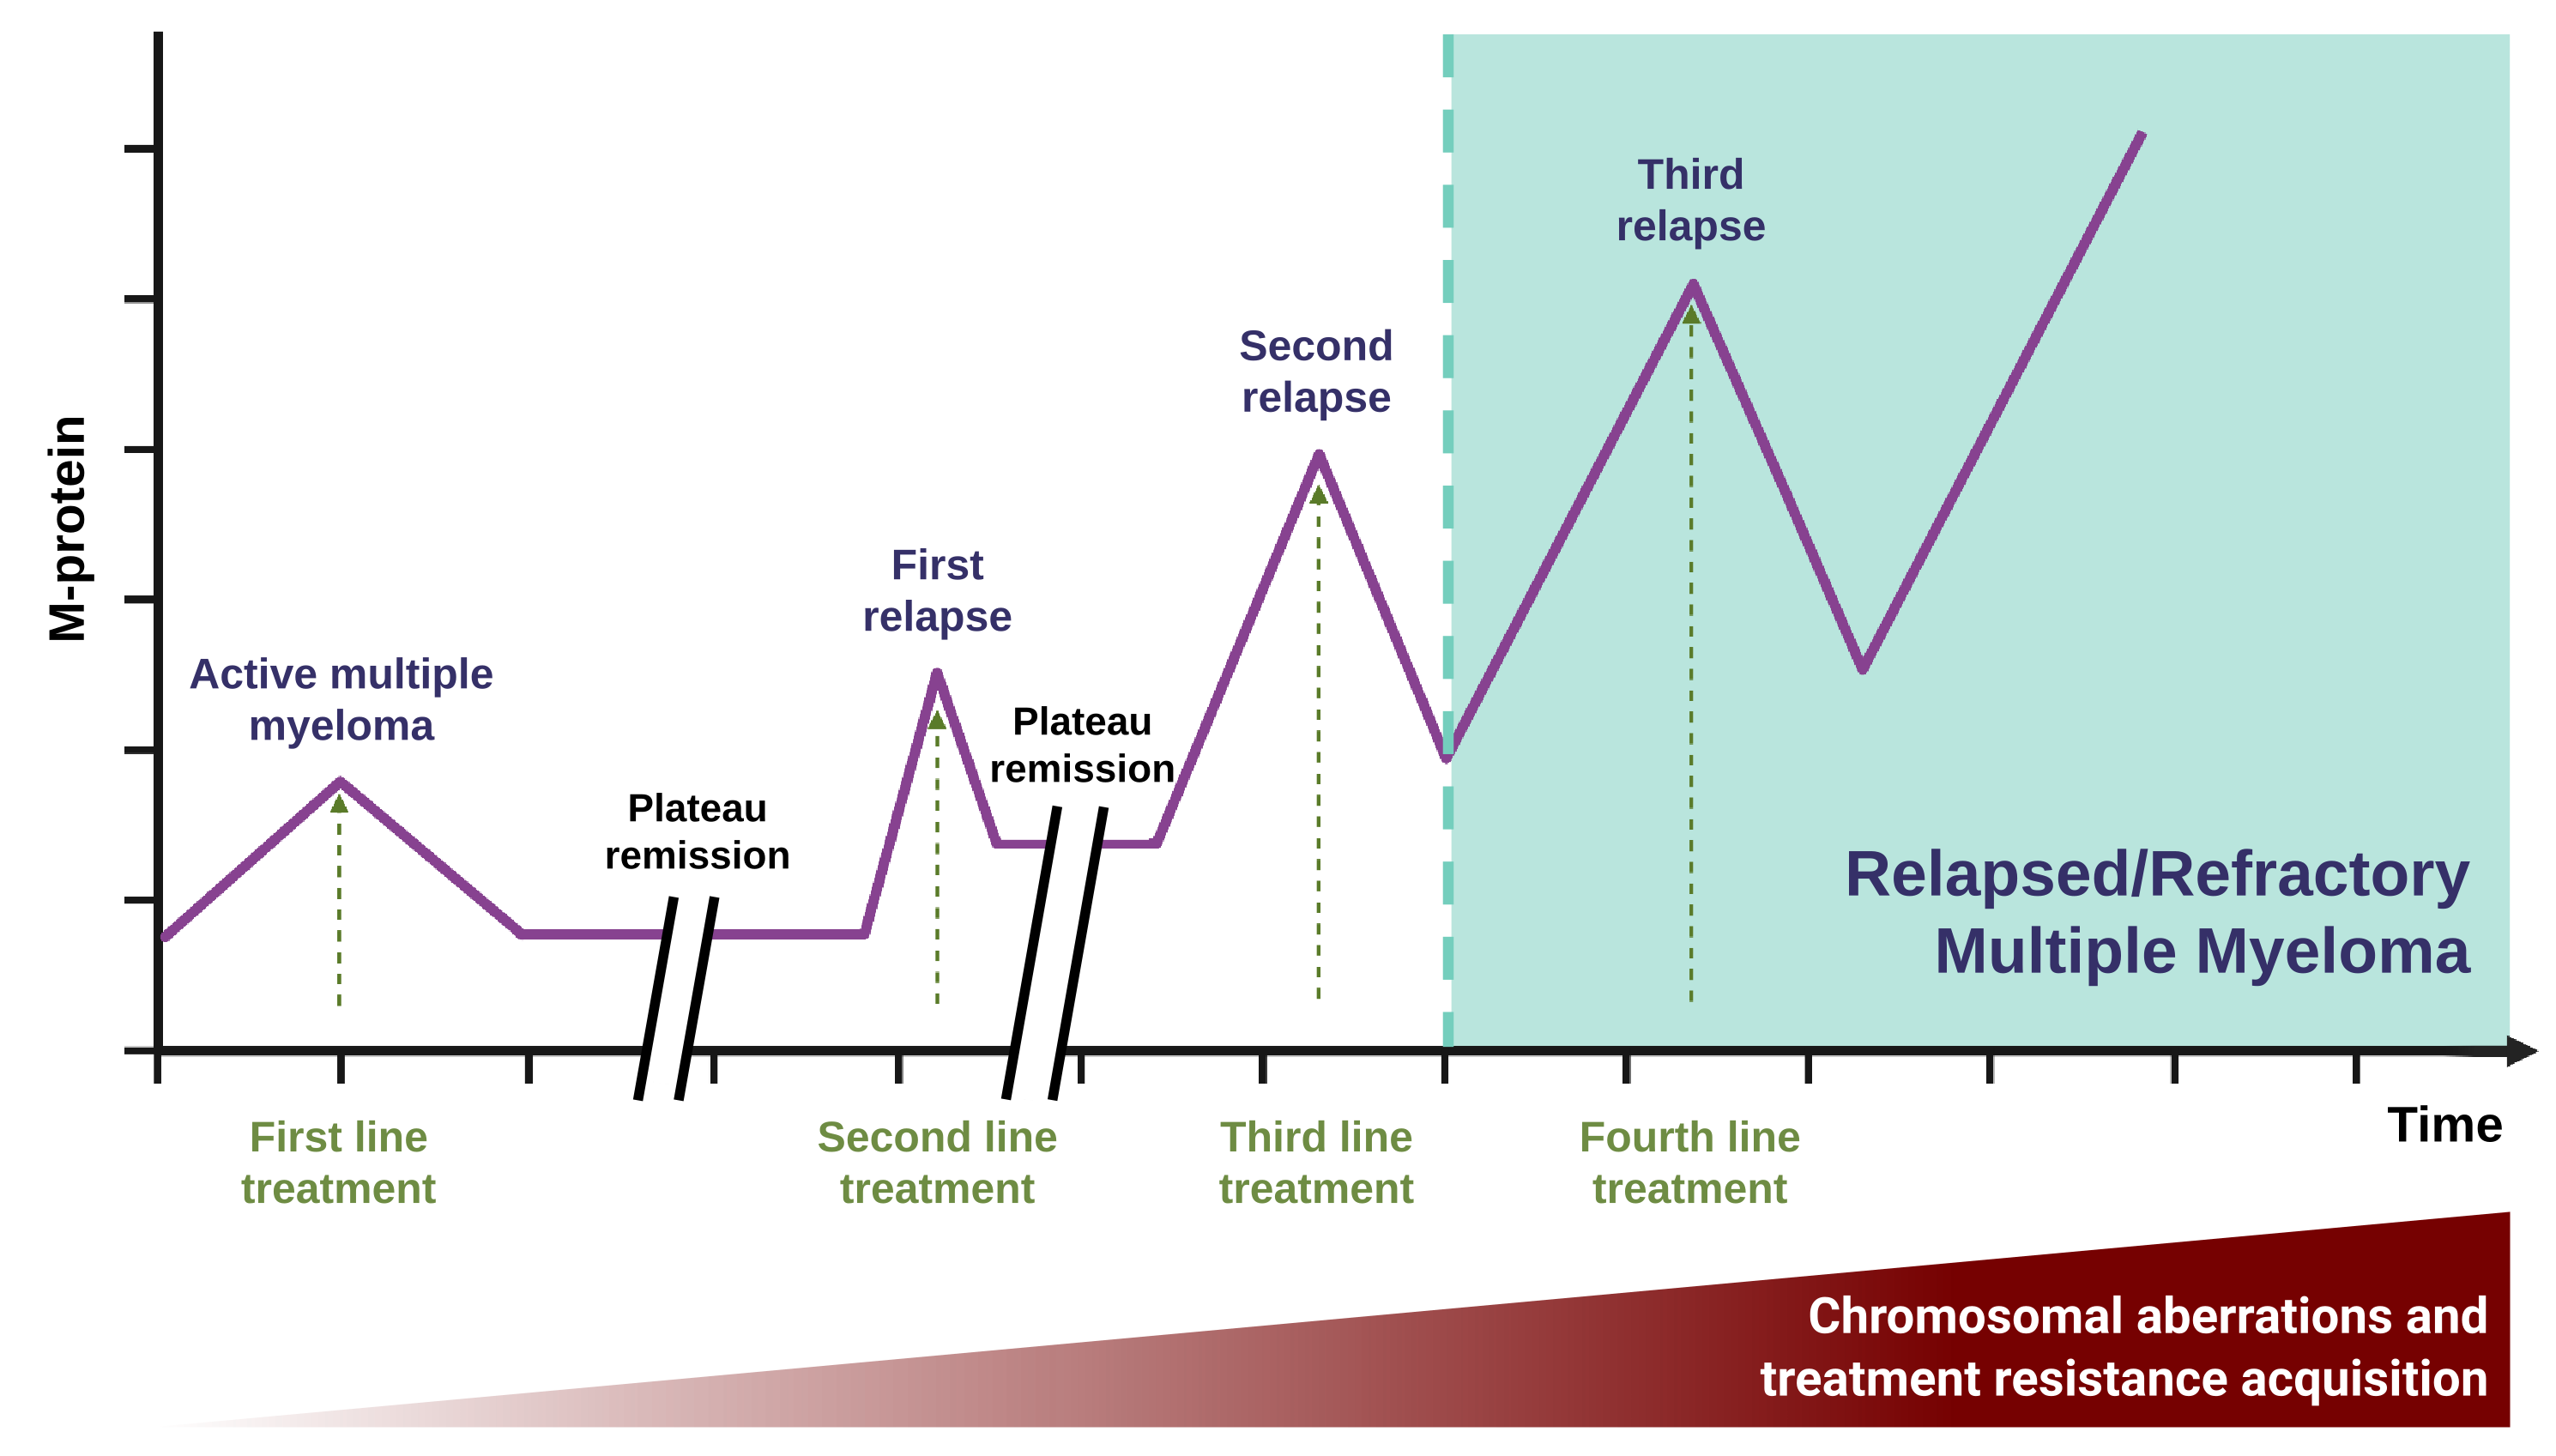
\includegraphics[width=0.8\textwidth]{img/evo_MM.png}
    \caption[Remission/relapse cycle of Multiple Myeloma]{Remission/relapse 
    cycle of MM. The disease trajectory is characterized by serial cycles of 
    response, remission, and relapse in the presence of treatment, typically 
    monitored through M protein levels (an abnormal antibody produced by 
    malignant plasma cells). Through successive relapses, MM cells acquire new 
    chromosomal abnormalities, leading to clonal evolution with diminished 
    depth and duration of response over time. Courtesy of Álvaro Otero Sobrino, 
    researcher of Hospital 12 de Octubre's Hematological Malignancies group.}
    \label{fig:evo_MM}
\end{figure}